


\chapter{L'aspect réseau}
Dans ce chapitre, les principales problématiques data centre dans un aspect réseau seront présentées et analysées. Seront abordées quelques questionnements sur les réseaux classiques pour l'essai de répondre aux nouveaux besoins data centres. Le chapitre présentera comment divers scénarios sont traités aujourd'hui et quels sont ses limites. 


\section{Le rôle du réseau dans les projets de TI}

Lors du développement de projets pour l'optimisation en \gls{ti} tels que la consolidation de data centres et la virtualisation de serveurs, une attention spéciale doit être prise au rôle critique des réseaux dans la planification, exécution et succès en général du projet. Il est souvent admet que des planifications supplémentaires par rapport aux réseaux auraient pu contribuer pour le succès de plusieurs projets.

%As organizations undertake information technology (IT) optimization projects, such as data center consolidation and server virtualization, they need to ensure that the proper level of focus is given to the critical role of the network in terms of planning, execution, and overall project success. While many consider the network early in the planning stages of these projects and spend time considering this aspect of these initiatives, many more feel that additional network planning could have helped their projects be more successful.


Les principaux types de changements réseau dans ces projets incluent l'implémentation d'équipement réseau supplémentaire pour augmenter ou améliorer la redondance, la capacité du réseau, la sécurité réseau et/ou la bande passante. Cependant, plusieurs requis associés à ces changements ne sont pas, en général, identifiés tout au début du projet. Très souvent ils ne sont pas détectés qu'après les étapes initiales du projet, imposant un supplément de travail et l'ajout des coûts non anticipés.

%The most common types of network changes in IT optimization projects include implementing new network equipment, adding greater redundancy, increasing capacity by upgrading switches, improving network security, and adding network bandwidth. However, many network requirements associated with these changes and the overall initiative are typically not identified until after the initial stages of the project and often require rework and add unanticipated costs. Regardless of project type, network challenges run the risk of contributing to increased project time lines and/or costs.


Les aspects réseau d'un projet peuvent être difficiles à gérer, et des critiques sur le fonctionnement général des réseaux sont fréquemment entendues. Des défis importants incluent la réalisation d'analyses des causes précises et opportunes, la compression de sa réactivité au niveau applicatif et la révélation des origines de problèmes de performance. Le simple achat d'équipement réseau n'aborde pas nécessairement ou proprement les requis réels.

%The networking aspects of projects can be challenging and user complaints about the network are frequently heard. Important challenges include the inability to perform accurate and timely root-cause analysis, understand application level responsiveness, and address network performance issues. Simply buying more network equipment does not necessarily or appropriately address the real requirements.


%Looking ahead, many expect that the network will become more important to their companies' overall success. To address this, networking investments related to support of server and storage virtualization are currently at the top of the list for consideration, followed by overall enhancement and optimization of the networking environment. To support virtualization of the entire IT infrastructure and to continue to optimize the network, IT organizations need to make architectural decisions in the context of the existing infrastructure, IT strategy, and overall business goals.


Pour supporter la virtualisation complète d'une infrastructure de \gls{ti} et continuer à optimiser le réseau, des décisions sur l'architecture doivent être faites dans le contexte de l'infrastructure existante, de la stratégie et objectifs amples du business. Sans le développement d'un plan réseau et la conception fonctionnelle associée, les transitions réseau peuvent être risquées et conduire à un contrôle réduit des services livrés, coûts potentiellement élevés contre des résultats insuffisants et des problèmes inattendus de performance ou disponibilité. 
%Developing a plan for the network and associated functional design is critical. Without a strong plan and a solid functional design, networking transitions can be risky, leading to reduced control of IT services delivered over the network, the potential for high costs with insufficient results, and unexpected performance or availability issues for critical business processes.


Traditionnellement un plan et conception fonctionnelle solides suffisaient pour augmenter le succès des projets avec un réseau réactif, optimisé, moins cher et répondant mieux aux engagements des services applicatifs. Alors que ce plan reste essentiel, il est difficile dans le contexte d'utilisation actuel de maitriser complètement  à l'avance la charge, dimension et tout autre requis qui doivent être assurés par les réseaux. On cherche plutôt à concevoir des architectures réseaux qui puissent s'étendre ou se rétracter ainsi que supporter des nouveaux services dynamiquement et rapidement  en fonctions des besoins immédiates. \cite{ibmPlanningVirtCCchap4}
%With a plan and a solid functional design, the probability of success is raised: a more responsive network with optimized delivery, lower costs, increased ability to meet application service level commitments, and a network that supports and fully contributes to a responsive IT environment.


\section{Éléments de base de l'architecture réseau}

\begin{figure}[h]
\begin{center}
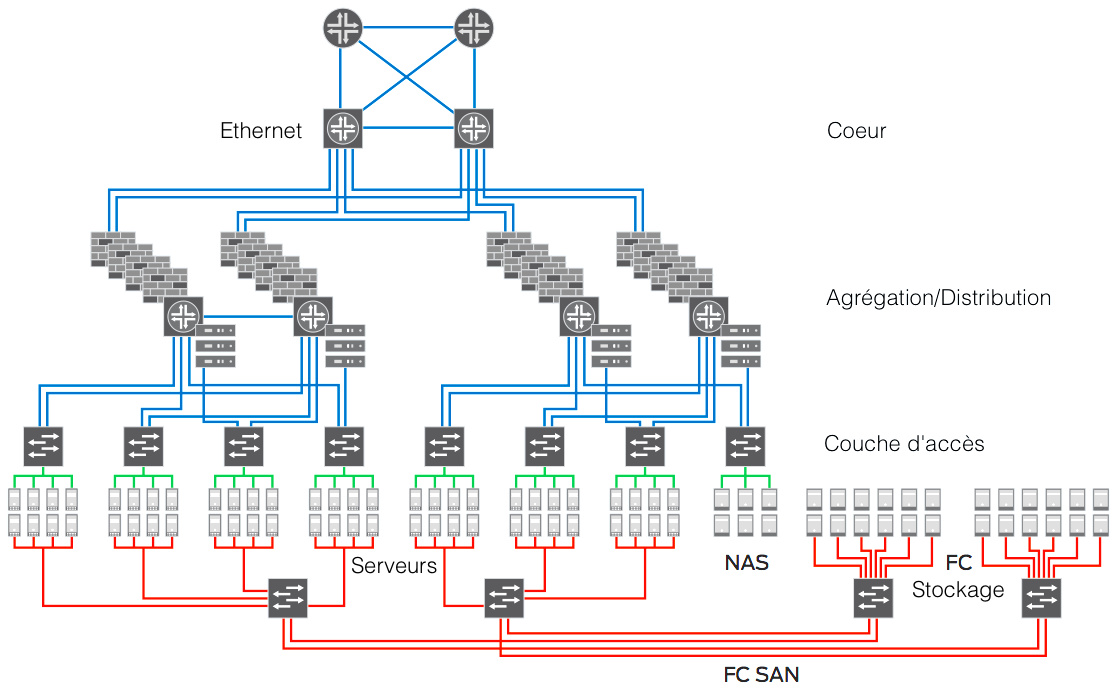
\includegraphics[width=0.98\textwidth]{images/LegacyNetworkArchitecture} 
\caption{Architecture réseau typique à trois niveaux. \cite{cloudReadyNetworkJuniper}}
\end{center}
\end{figure}

\section{Challenges réseau}

Unified Fabric

If one studies a typical data center server infrastructure, it is easy to notice that servers have a series of network interfaces connected to multiple types of networks (LAN, SAN, IPC). This arrangement adds complexity in the form of cost, cabling, port count, scalability, power, and cooling. If we follow the same tradition in a cloud data center, this architecture will not scale to the density that is typically expected. Hence, to continue to reduce the total cost of ownership (TCO) and to deploy virtual machines, all servers must have a consistent and ubiquitous set of network and storage capabilities. One of the simplest and most efficient ways to deliver these capabilities is to deploy a unified fabric. The shift to a unified fabric gives all servers (physical and virtual) access to the LAN, SAN, and IPC networks, allowing more to be consolidated in the customer’s network for greater efficiency and costs savings.

Cisco is offering not only 10 Gigabit Ethernet, but also lossless 10 Gigabit Ethernet, currently called Data Center Ethernet or Enhanced Ethernet. This becomes the foundation to consolidate fabrics like Fiber Channel (for SAN), which require the stringent lossless nature of a network. Fibre Channel over Ethernet (FCoE), which is a standard accepted by standard bodies and industry, is leading the way to unify fabric on a cloud data center. Hence, to consolidate server I/O, the server access layer must be adapted to support a unified fabric. Additionally, a new breed of adapters, called converged network adapters (CNAs), would be implemented in the server platform, which will act at the consolidation and virtualization point in the compute layer.


Cisco believes that the network platform is a foundational component of a utility service platform as it is critical to providing intelligent connectivity within and beyond the data center. With the right built-in and external tools, the network is ideally placed to provide a secure, trusted, and robust services platform.

The network is the natural home for management and enforcement of policies relating to risk, performance, and cost. Only the network sees all data, connected resources, and user interactions within and between clouds. The network is thus uniquely positioned to monitor and meter usage and performance of distributed services and infrastructure. An analogy for the network in this context would be the human body’s autonomic nervous system (ANS) that acts as a system (functioning largely below the level of consciousness) that controls visceral (inner organ) functions. ANS is usually divided into sensory (affer- ent) and motor (efferent) subsystems that is analogous to visibility and control capabili- ties we need from a services platform to derive a desired outcome. Indeed, at the time of this writing, there is a lot of academic research into managing complex network systems, might they be biological, social, or traditional IT networking. Management tools for the data center and wider networks have moved from a user-centric focus (for example, GUI design) to today’s process-centric programmatic capabilities. In the future, the focus will most likely shift toward behavioral- and then cognitive-based capabilities.

The network also has a pivotal role to play in promoting resilience and reliability. For example, the network, with its unique end-to-end visibility, helps support dynamic orchestration and redirection of workloads through embedded policy-based control capabilities. The network is inherently aware of the physical location of resources and users. Context-aware services can anticipate the needs of users and deploy resources appropriately, balancing end-user experience, risk management, and the cost of service.


\section{Différents usages}

\section{Agilité}

\section{Sécurité}

introduction
Some security risks unique to a virtualization infrastructure include communication blind spots, inter-VM attacks, and mixed trust level VMs. Instant-on gaps and resource contention are also important considerations. This section addresses each of these threats and issues.

communication Blind Spots

In virtualized environments, traditional network security appliances are blind to the communication between VMs on the same host unless all communications are routed outside the host machine to this separate appliance. But this security configuration introduces significant time lags. One way to eliminate blind spots while reducing time lags is to place a dedicated scanning security VM on the host that coordinates communication between VMs. This solution works well in a virtualized environment. However, a dedicated security VM is not ideal for a cloud environment. The dedicated security VM integrates with the hypervisor to communicate with other guest VMs. In some cloud environments, such as in a multi-tenant public cloud, users do not have access to the hypervisor. In the cloud, protection is best provided as self-defending VMs. Protection is self contained on each VM and does not require communication outside of the VM to remain secure.

inter-Vm attacks and hypervisor compromises

Virtualized servers use the same operating systems, enterprise applications, and web applications as physical servers. Hence, the ability of an attacker to remotely exploit vulnerabilities in these systems and applications is a significant threat to virtualized environments as well. And once an attacker compromises one element of a virtual environment, oather elements may also be compromised if virtualization-aware security is not implemented.
In one scenario, an attacker can compromise one guest VM, which can then pass
the infection to other guest VMs on the same host. Co-location of multiple VMs
increases the attack surface and risk of VM-to-VM compromise. A firewall and an intrusion detection and prevention system need to be able to detect malicious activity at the VM level, regardless of the location of the VM within the virtualized environment.

Another attack mode involves the hypervisor, which is the software that enables multiple VMs to run within a single computer. While central to all virtualization methods, hypervisors bring both new capabilities and computing risks. A hypervisor can control all aspects of all VMs that run on the hardware, so it is a natural security target. Therefore, securing a hypervisor is vital, yet more complex than it seems.

In an attack known as “hyperjacking,” malware that has penetrated one VM may attack the hypervisor. When a guest VM attempts this attack, it is often called a “guest VM escape” because the guest VM breaks out of, or escapes, its isolated environment and attacks the host hypervisor. Once compromised, a hypervisor can then attack other guest VMs on that host.

VMs make requests to the hypervisor through several different methods, usually involving a specific application programming interface (API) call. An API is the interface created to manage VMs from the host machine. These APIs are prime targets for malicious code, so virtualization vendors attempt to ensure that APIs are secure and that VMs make only authentic (i.e. authenticated and authorized) requests. Because this is a critical path function, speed is a significant requirement in all hypervisors to ensure that overall performance is not impeded.
When attackers targeted a zero-day vulnerability in a virtualization application called HyperVM made by LXLabs, as many as 100,000 web sites were destroyed [1]. In addition, certain virtualization vendors like Amazon Web Services have made their APIs public. These will undoubtedly become interesting targets for cybercriminals. Vendors that have not made their APIs public like vSphere, while not usually externally exposed, can also become potential targets for attacks within their perimeters. There is a risk that, owing to the rapid change in the API space and the current race to market, virtualization management systems will not be secure in the future.

mixed trust level Vms

VMs with mission-critical data may reside on the same host as VMs with less critical data – resulting in mixed trust level VMs. Enterprises can attempt to segregate these different levels of secure information on separate host machines, but in some cases, this can defeat the purpose of a virtualized environment – to make the most efficient use of resources. Enterprises need to ensure that mission-critical information is protected while still realizing the benefits of virtualization. With self-defending VM security, VMs can remain safe even in mixed trust level environments, with protection such as intrusion detection and prevention, a firewall, integrity monitoring, log inspection, and antivirus capabilities.

instant-on gaps

Virtualized environments are not necessarily inherently less secure than their physical counterparts. However, in some cases, the practical uses of virtualization can introduce vulnerabilities, unless administrators are aware of these vulnerabilities and take steps to eliminate them. Instant-on gaps are an example of such a vulnerability.
Beyond server consolidation, enterprises take advantage of the dynamic nature of VMs by quickly provisioning, cloning, migrating, and decommissioning VMs as needed, for test environments, scheduled maintenance, and disaster recovery, and to support task workers who need computational resources on-demand. As a result, when VMs are activated and inactivated in rapid cycles, rapidly and consistently provisioning security to those VMs and keeping them up-to-date can be challenging.

After a period of time, dormant VMs can eventually deviate so far from the baseline security state that simply powering them on introduces significant security vulnerabilities. And even if VMs are dormant, attackers may still be able to access them. Also, new VMs may be cloned from VM templates with out-of-date security. Even when VMs are built from a template with virus protection and other security applications, the VMs need the security agent to have the latest security configurations and pattern file updates.

When dormant, reactivated, or cloned VMs have out-of-date security, attackers may be able to leverage an exploit for a longer period of time – the attack may have more longevity. Generally, if a guest VM is not online during the deployment or updating of antivirus software, it will lie dormant in an unprotected state and be instantly vulnerable when it does come online. One solution is a dedicated security VM on each host that automatically updates VMs with the latest security when activated or cloned, and safely allows enterprises to realize the benefits of virtualization.

resource contention 

%When resource intensive operations such as regular antivirus scans and pattern file updates designed for physical environments are applied to VMs, these operations can quickly result in an extreme load on the system. When antivirus scans or scheduled updates simultaneously kick into action on all VMs on a single physical system, the result is an antivirus storm. This storm is like a run on the bank, where the bank is the underlying virtualized resource pool of memory, storage, and CPU. This performance impact hampers server applications and VDI environments.

The legacy security architecture also results in linear growth of memory allocation as the number of VMs on a single host grows. In physical environments, antivirus software must be installed on each operating system. Applying this architecture to virtual systems means that each VM requires additional significant memory footprint  an unwanted drain on server consolidation efforts.
Products that are not virtualization-aware suggest the use of randomization or grouping to avoid resource contention.

However, randomization does not help to avoid times of high system usage and requires that a long period of time be reserved for the full scan cycle. Grouping does not allow for the mobile nature of virtualization, requiring reconfiguration when VMs are migrated or cloned.



